
The field of computational neutronics, computationally solving the Boltzmann Transport equation applied to neutrons (transport equation), is generally concerned with modeling neutrons in a nuclear system. These systems include nuclear reactors or shielding problems where there exists a fixed source of neutrons. The materials used in these systems have a variety of properties, including how they effect the energy of the neutron. Many materials that are commonly used in nuclear applications, particularly those containing hydrogen, exhibit a property known as upscattering, where lower energy neutrons are ``bounced" to higher energies. The details of scattering can dramatically impact which numerical methods to choose, particularly when solving the transport equation deterministically. 

% This comes a bit too soon. You need to tell us you're solving the transport equation, that you're doing that deterministically, and that energy groups are a thing. Having this in the first paragraph is before we're ready for it. 
%Mathematically, a scattering matrix representing the scattering cross sections from group $\rg$ to $\rg'$ with the highest energy in group 1 and the lowest in group $G$ would be lower triangular if there is no upscattering. The entries $[\rg, \rg'\geq \rg]$ account for downscattering. A triangular matrix has nice computational properties that make the solving of the problem easier. However, when upscattering is present, the triangularity of the matrix is broken and other solution techniques must be employed. The most commonly used method in neutron transport calculations for problems with upscattering is known as the Gauss-Seidel Method. 
% This whole paragraph should go somewhere else. It's also confusing and not quite right. 

% Instead, you might want to add a paragraph about impact and more broadly motivating this work. 

In this work, we explore methods for speeding up nonlinear diffusion acceleration (NDA) in the presence of upscattering. NDA is also known as coarse-mesh finite difference and is a well-known technique applied to accelerate the scattering convergence in neutronics calculations. In multigroup neutronics problems, NDA is effective in conjunction with Gauss Seidel (GS) iteration in energy if there is little upscattering. However, when upscattering has a significant impact, which is common with thermal systems, the efficiency of GS-NDA degrades as extra iterations are required for convergence in energy \cite{park-nda}.

To remedy the issue in GS with upscattering, an energy two-grid (TG) acceleration scheme was first developed to approximate iteration error by solving a one-group diffusion-like equation with artificial material properties generated by using the scattering eigen-spectrum \cite{morel-upscat}. Later, a transport TG (TTG) method was developed that approximates the energy error using a consistent \sn\ solver in multi-D \cite{evans-upscat}. [need a statement here about why these either don't work with NDA or are insufficient st we need a new method]. Inspired by the previous studies, we derive a TG scheme for the NDA equation with GS iteration.

% you need to flip the order of the TE section and previous work. Previous work mostly doesn't make any sense without seeing the TE and how it's discretized. The opening section barely makes sense. 

\section{Previous Work}
% we definitely don't have enough information to understand this paragraph, even after the TE section. Please rewrite. 
To accelerate the convergence of source iteration, a method that converges the flux inside of a given enegy group, Nonlinear Diffusion Acceleration was developed \cite{Knoll2011} \cite{park-nda}. 
% Not sure if this is the right way to do it, but you haven't told us what SI is. 
NDA pairs a lower order equation with a higher order, drift diffusion equation. 
% we also don't know what a drift diffusion equation is. 
As the higher order equation is not conservative, the method is formally inconsistent: the scalar flux and current may not be equal upon convergence,
%  equal to one another? Should they be? That doesn't make any sense to me. Or, the scalar flux and current in the higher order isn't equal to NDA? Please clarify.
% Also, make sure to tell us what the scalar flux and current are.
although they are equal in the limit as the spatial mesh is refined. However, second order accuracy
% which thing has second order accuracy? This also came out of nowhere
 can still be maintained with the high-order equation generally giving a more accurate shape and the conservative low-order equation giving a more accurate magnitude.
 % you never told us the low order equation is conservative.  
 The combination of the two equations has been found to be more accurate than either equation alone \cite{morel-holo}.
 
Since its development, NDA has been tried with a variety of higher order equations, \cite{morel-holo}\cite{Wang2013} as well as spatial discretizations \cite{morel-holo}\cite{Schunert2017}. In this work, we explore NDA with the Self-Adjoint Angular Flux Equation (SAAF) and a continuous finite element discretization.

% the following paragraph is useful context. Needs to come earlier. 
The steady-state transport equation is dependent on space, angle, and energy. It is often solved via a series of nested iterations. The various iteration methods and how they are used with each other are described in detail in Ch. \ref{sec:iterative}. The Nonlinear Diffusion Acceleration happens in the source iteration, where angle and energy are fixed. When energy is discretized into more than one energy group, an outer layer of iteration is introduced. One of the most commonly-used methods for iterating over energy groups is known as Gauss Seidel. Gauss Siedel is guaranteed to converge; however, in problems with significant upscattering, the time it takes to reach convergence can become arbitrarily slow. 
% probably need a citation for that claim.

A number of techniques to accelerate Gauss Seidel convergence have been developed \cite{morel-upscat} \cite{evans-upscat}, although to our knowledge none have yet been paired with NDA. The primary techniques used in commercial transport software rely on a rebalance scheme and coarse-mesh finite-difference diffusion.
% I'm not sure we can understand what that means either. 
Although these methods are widely used and successful for acceleration, they are very sensitive to the coarse mesh size. Rebalancing with too fine a mesh may be divergent, and an overly coarse mesh degrades performance \cite{evans-upscat}.

While for standard problems, the proper mesh size is generally well understood;
% I don't know what is a standard problem; shielding isn't non-standard...???
 this is not the case for shielding problems. Adams and Morel developed an upscatter acceleration scheme known as the Two-Grid method. An estimation of the error at each Gauss Seidel iteration is calculated using a collapsed in energy, one-group diffusion equation and energy eigenvector of the Gauss Seidel iteration matrix. These
 % I don't know what "these" means here
  make up the correction term to the scalar flux at each group, which is applied at each iteration. In one dimensional calculations, Adams and Morel have demonstrated their method to be very efficient for thermal upscattering problems \cite{morel-upscat}.

\section{The Boltzmann Transport Equation}
The angular neutron flux of a reactor, $\psi$ can be found by solving the steady state Boltzmann Transport equation,
%
\begin{equation}
\begin{split}
 [\hat{\Omega} \cdot \nabla + &\Sigma(\vec{r}, E)]\psi(\vec{r}, \hat{\Omega}, E) = \chi(E) \int_0^\infty dE' \nu \Sigma_{f}(\vec{r}, E') \int_{4\pi} d\hat{\Omega}'\psi(\vec{r}, \hat{\Omega}', E') \\   &+ \int_0^\infty dE' \int_{4\pi} d\hat{\Omega}' \Sigma_s(\vec{r}, E' \rightarrow E, \hat{\Omega}' \cdot \hat{\Omega})\psi(\vec{r}, \hat{\Omega}', E') + Q(\vec{r}, \hat{\Omega}, E)   \:,
\end{split}
\label{eq:transport}
\end{equation}


where $\hat{\Omega}$ represents the angle; $\vec{r}$, the position vector; $E$, the energy; $\Sigma$, the total macroscopic cross-section; $\Sigma_f$, the macroscopic fission cross-section; $\Sigma_s$, the macroscopic scattering cross section; $\chi$, the fission energy distribution; $\nu$, the average number of neutrons per fission; and $Q$, an external source. 

In this work, we apply an incident boundary condition, where for $\hat{n} \cdot \hat{\Omega} < 0$, with $\hat{n}$ being the outward normal on the boundary $\partial \mathcal{D}$,
\begin{equation}
    \psi(\vec{r}, \hat{\Omega}, E) = \psi^{inc}(\vec{r}, \hat{\Omega}, E), \hspace{5mm} \vec{r} \in \partial \mathcal{D}\:,
\end{equation}
though other boundary conditions such as reflecting, periodic, and vacuum are valid.

\subsection{Forms of the Transport Equation}
There are are several forms of the transport equation that are of interest in the field of nuclear energy. 

\subsubsection{Fixed Source Form}
To write Eqn.~\eqref{eq:transport} in a fixed source form, we drop the fission term and retain the source, $Q$. If there is fission in the system, fission neutrons can be included in the source term. We use the same boundary conditions as above. 
%
\begin{equation}
\begin{split}
 [\hat{\Omega} \cdot \nabla + \Sigma(\vec{r}, E)]\psi(\vec{r}, \hat{\Omega}, E) &= \\ \int_0^\infty dE' &\int_{4\pi} d\hat{\Omega}' \Sigma_s(\vec{r}, E' \rightarrow E, \hat{\Omega}' \cdot \hat{\Omega})\psi(\vec{r}, \hat{\Omega}', E')  + Q(\vec{r}, \hat{\Omega}, E)
\end{split}
 \label{eq:transport_fixed_source}
\end{equation}

\subsubsection{$k$-Eigenvalue Form}
When fission is in a system, we are often interested in the multiplication behavior, which can be described by a parameter, $k$, the ratio of neutrons in two successive generations. If the chain reaction is self-sustaining and time-independent, the reactor is known as ``critical" and $k=1$. A $k>1$ gives an increasing population, termed supercritical, and $k<1$ gives a subcritical, decreasing population. We scale $\nu$ in Eq. \eqref{eq:transport} by $k$ to express the deviation from critical. This gives the following equation,
%
\begin{equation}
    \label{eq:transport_eigenvalue}
    \begin{split}
        [\hat{\Omega} \cdot \nabla + \Sigma(\vec{r}, E)]\psi(\vec{r}, \hat{\Omega}, E) &= \frac{\chi(E)}{4\pi k} \int_0^\infty dE' \nu \Sigma_{f}(\vec{r}, E') \int_{4\pi} d\hat{\Omega}'\psi(\vec{r}, \hat{\Omega}', E') \\ &+ \int_0^\infty dE' \int_{4\pi} d\hat{\Omega}' \Sigma_s(\vec{r}, E' \rightarrow E, \hat{\Omega}' \cdot \hat{\Omega})\psi(\vec{r}, \hat{\Omega}', E') \ :,
    \end{split}
\end{equation}
where the $\frac{1}{4\pi}$ is added to represent that fission neutrons are born isotropically. We again using the same boundary conditions. 

Eqn.~\eqref{eq:transport_eigenvalue} is an eigenvalue problem that, with some algebraic manipulation, can be written of in the form $A\psi = \frac{1}{k} F\psi$ and solved via standard eigenvalue solvers. 

In this work, we present all methods in fixed-source form; however, they can all be easily extended to $k$-eigenvalue form for criticality calculations. 

\section{Space-Angle Approximations of Interest}
There are many simplifications and approximations that can be made to facilitate the solution of the transport equation. In this work, we assume our scattering and fixed sources are isotropic, which gives the following form
%
\begin{equation}
\begin{split}
 [\hat{\Omega} \cdot \nabla + \Sigma(\vec{r}, E)]\psi(\vec{r}, \hat{\Omega}, E) &= \\ \frac{1}{4\pi}  \int_0^\infty &\Sigma_s(\vec{r}, E' \rightarrow E)  dE' \int_{4\pi} d\hat{\Omega}'\psi(\vec{r}, \hat{\Omega}', E')  + \frac{1}{4\pi}Q \:.
\end{split}
 \label{eq:transport_isotropic_scattering}
\end{equation}
%
This equation gives the angular flux. To find the scalar flux, $\phi$, which is often the quantity desired in practice at it is used to give the reactions rates needed for engineering solutions, we must integrate over all directions
\begin{equation}
    \phi(\vec{r}, E) = \int_{4\pi} \phi(\vec{r}, \hat{\Omega}, E) d \Omega \:.
\end{equation}

\subsection{Self-Adjoint Angular Flux}
Discretizing the traditional transport equation, Eqn.~\eqref{eq:transport_isotropic_scattering}, in space, particularly using the finite element method, presents a number of challenges \cite{saaf}. A finite element spatial discretization is generally favorable as it produces as symmetric positive-definite (SPD) linear system. SPD systems can be solved using a number of well-studied, robust solution techniques. In order to make use of these properties, we must rearrange the standard transport equation into a form that is more computationally friendly, a self-adjoint form \cite{saaf}.

The monoenergetic version of the Self-Adjoint Angular Flux equation appropriate for $S_N$ calculations is 
% you didn't tell us what an SN calculation is yet
\begin{equation}
    - \vec{\Omega} \cdot \nabla \frac{1}{\Sigma_t}\vec{\Omega} \cdot \nabla \psi + \Sigma_t \psi = \frac{1}{4\pi}[\Sigma_s\phi + Q - \vec{\Omega} \cdot \nabla \frac{(\Sigma_s\phi + Q)}{\Sigma_t}]\:.
    \label{eq:SAAF}
\end{equation}
% do you use the monoenergetic form? This section feels a little out of nowhere. Maybe an additional sentence or two telling us why you're telling us this out of every possible spatial discretization form. 


\subsection{The Diffusion Equation}
To simplify even further, we employ a commonly-used approximation known as the diffusion equation. To derive the diffusion equation, we consider the neutron balance within an infinitesimal volume centered at a point, $r$. For simplicity of notation,we will present this derivation assuming all neutrons have the same energy. Under steady state conditions, neutron conservation requires
%
\begin{equation}
    \textit{neutrons leaking out} + \textit{neutrons absorbed} = \textit{source neutrons emitted}.
\end{equation}
We describe the neutrons leaking out as the rate of the current, $J$, in all directions, the neutrons absorbed is the absorption cross section times the scalar flux, $\Sigma_a\phi$, and the source neutrons are represented by the source variable, $Q$. 
\begin{equation}
    \nabla\cdot \vec{J}(\vec{r}) + \Sigma_a(\vec{r})\phi(\vec{r}) = Q(\vec{r})
\end{equation}
Using Fick's Law which relates the current to the flux, $\vec{J}(\vec{r}) = -D(\vec{r})\nabla\phi(\vec{r})$ where $D = 1/3\Sigma_t$, we get the diffusion approximation

\begin{equation}
\begin{split}
 - \nabla \cdot D(\vec{r})\nabla\phi(\vec{r}) &+ \Sigma_a \phi(\vec{r}) = Q(\vec{r}).
\end{split}
\label{eq:diffusion_fixed_source}
\end{equation}

While the diffusion equation is much easier to solve, due to the assumptions made in the Fick's Law approximation, it is not valid near boundaries where material properties change dramatically, near localized sources, or in strongly absorbing media \cite{lewis-miller}.

\subsection{Nonlinear Diffusion Acceleration}
This work presents an acceleration to a method known as Nonlinear Diffusion Acceleration (NDA). NDA reformulates the transport equation as a correction to the diffusion equation and uses a two step process to solve. For reference, we repeat the derivation of the low-order NDA equation found in \cite{morel-holo} with small modifications assuming no fission source and vacuum boundary conditions. Consider the first order, one-group, fixed-source, steady-state \sn transport equation with isotropic scattering. 

  \begin{equation}
  \vec{\Omega}\cdot \nabla \psi \left(\vec{r}\right)+ \Sigma_{\mm{t}}\left(\vec{r}\right)\psi = \frac{1}{4 \pi} \Sigma_{\mm{s}}\left(\vec{r}\right) \phi\left(\vec{r}\right) + \frac{1}{4 \pi} Q\:.
  \end{equation}
Integrate over all angles to obtain the zeroth moment equation
\begin{equation}
  \nabla \cdot \vec{J} + \Sigma_a\phi  =  Q
  \label{eq:zeroth_moment_1g}
  \end{equation}
where $\vec{J} = \int_{4\pi} \vec{\Omega}\psi$ and $\Sigma_a$ is the absorption cross section.   Now consider the first moment equation:
  \begin{equation}
  \nabla \cdot \overset{\text{\scriptsize$\leftrightarrow$}}{P} + \Sigma_t J = 0
  \end{equation}
where $\nabla \cdot \overset{\text{\scriptsize$\leftrightarrow$}}{P} =  \int_{4\pi} \vec{\Omega} \vec{\Omega} \cdot \nabla \psi$. It can be rewritten as: 

  \begin{equation}
  J= -\frac{1}{\Sigma_t} \nabla \cdot \overset{\text{\scriptsize$\leftrightarrow$}}{P}. 
  \end{equation}
  By adding and subtracting the diffusion coefficient, $D = \frac{1}{3\Sigma_t}$, times the gradient of the flux, it takes the form of a correction to Fick's Law. 
  \begin{equation}
  J = -D \nabla \phi + D \nabla \phi - \frac{1}{\Sigma_t} \nabla \overset{\text{\scriptsize$\leftrightarrow$}}{P} \\
  = -D \nabla \phi - \vec{\textbf{D}} \phi
  \label{eq:fick_corr_1g}
  \end{equation}
  where 
 \begin{equation}
  \vec{\textbf{D}} (\psi) = \frac{\int_{4\pi} [\frac{1}{\Sigma_t} \vec{\Omega} \vec{\Omega}\cdot \nabla \psi] - D \nabla \phi^{ho}}{\phi^{ho}}.
  \label{eq:drift_vector}
  \end{equation} 
Where $\psi^{ho} = \int_{4\pi} \psi(\Omega, \vec{r}) d\Omega$ where $\psi$ is the solution of the higher order equation. Plugging \eqref{eq:fick_corr_1g} into \eqref{eq:zeroth_moment_1g} we have the following NDA equation:
  \begin{equation}
  \nabla\cdot(-D \nabla \phi - \vec{\bf D} \phi) + \Sigma_a \phi = Q \:. \label{eq:NDA_1g}
  \end{equation}
  
Because NDA uses the solution from a higher-order in calculating the drift vector, it will not give an exact correction. While NDA maintains much of the accuracy of the higher-order equation when compared to diffusion, the two are not exactly equal. 


\subsection{Coupling NDA and SAAF}
In this work, we use SAAF as the higher order equation and NDA to accelerate the convergence of source iteration. The implementation of the algorithm is outlined below:

\begin{enumerate}
    \item Intitialize system, by setting $\vec{\textbf{D}}$ to 0 and solving \eqref{eq:NDA_1g} to get $\phi^0$ 
    \item Loop Until Convergence:
        \begin{enumerate}
            \item Solve \eqref{eq:SAAF} for $\psi^l$ using $\phi^{l-1}$ on RHS.
            \item Calculate drift vector, \eqref{eq:drift_vector}, using $\psi^l$
            \item Solve \eqref{eq:NDA_1g} for $\phi^l$
            \item Check $\phi^{l-1}, \phi^l$ for convergence
        \end{enumerate}
    \item Return $\phi$
\end{enumerate}

While we are able to replicate the results of \cite{Wang2013}, showing a significant reduction in the number of source iterations necessary when using NDA with SAAF as compared to SAAF alone, NDA only acclerates one layer of iteration. The presence of upscattering introduces another layer of iteration: Gauss-Seidel iteration in energy. In the following section we derive an acceleration scheme for the outer layer of iteration.


\section{Methods of Discretization}
The angular flux, $\psi$, is a function of space, angle, and energy. In the solution process, each one of those dimensions is discretized. There are several choices that have to be made regarding discretizations. In this work, we endeavor to show equation forms that are discretization agnostic as well as showing formulations unique to the particular discretization methods we chose to implement. 

\subsection{Angular Discretization}

Angular discretization on the left hand side of \eqref{eq:transport} is handled via the discrete ordinates ($S_N$) method, a finite-element collocation method \cite{Lathrop1965}. We assume the sources are isotropic and do not perform any additional expansion, however they can be expanded via Spherical Harmonics and the methods will still hold. 

\begin{figure}[H]
    \centering
    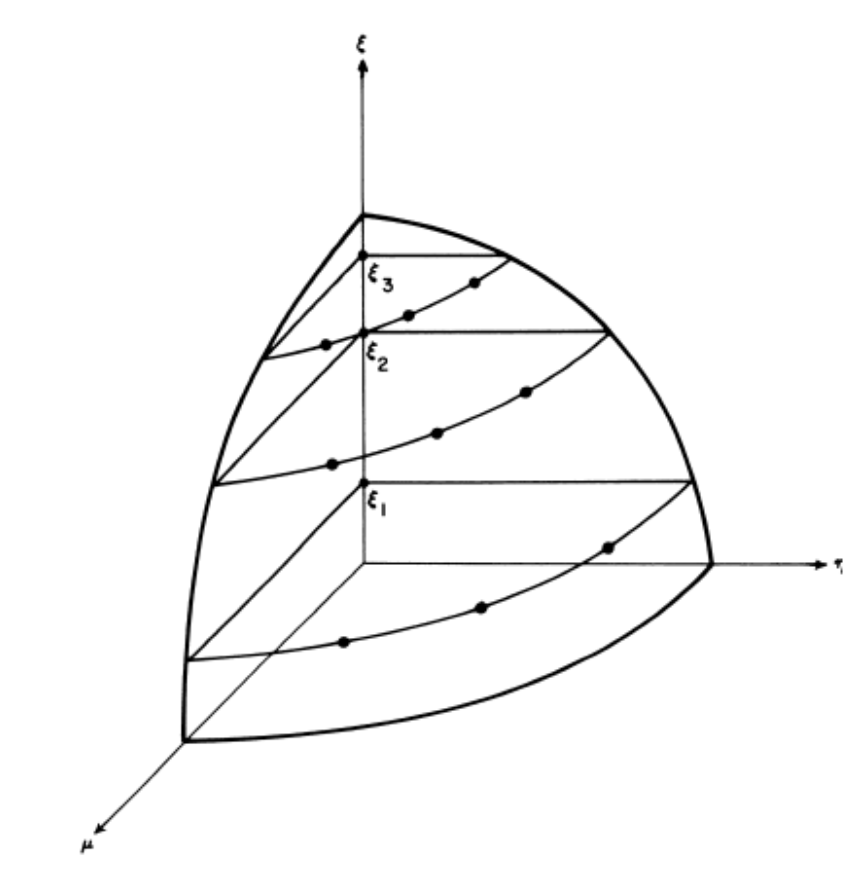
\includegraphics[width=.5\textwidth]{fig/SNPoints.png}
    \caption{Equally-Weighted Gauss-Chebyshev Quadrature Points \cite{Lathrop1965}}
    \label{fig:SN}
\end{figure}

The $S_N$ method evaluates the equation at number of discrete angles or ``ordinates" and then sums over all angles with their given weights to perform a quadrature. To choose quadrature points, an octant of the unit sphere is discretized into several levels. At each level several nodes are chosen. We use a Gauss-Chebyshev angular quadrature set, which can be thought of as a product set, combining a one dimensional Gaussian Quadrature along the polar angles and an equally-weighted Chebyshev quadrature along the azimuthal angles \cite{jarrel-thesis}. For a set of angles, $M$, a function integrated in angle is discretized as follows:

\begin{equation}
\int \Omega f(\Omega) d\Omega = \sum\limits_{\mrm=1}^{M} w_\mrm f_\mrm.    
\end{equation}






The discretized, steady-state, $S_N$ transport equation is given as follows,

 \begin{equation}
  \vec{\Omega}_\mrm \cdot \nabla \psi_\mrm \left(\vec{r}\right)+ \Sigma_{\mm{t}}\left(\vec{r}\right)\psi_\mrm = \frac{1}{4 \pi} \Sigma_{\mm{s}}\left(\vec{r}\right) \phi\left(\vec{r}\right) + \frac{1}{4 \pi} Q
  \label{eq:transport-angular}
 \end{equation}
where $\mrm$ is the angular index and $\phi = \sum\limits_{\mrm=1}^M \omega_\mrm \psi_\mrm$.

\subsection{Energy Discretization}
In our treatment of energy, we divide the full energy spectrum into several energy groups. By convention, the highest energy group is given the index, 1, with the index number going up until it reaches the lowest energy group. In expanding to multiple energy groups, we must take into account scattering from one group, $\rg'$ to another, $\rg$, denoted as $\rg' \rightarrow \rg $. 

The energy discretized, steady-state, transport equation is

 \begin{equation}
  \vec{\Omega} \cdot \nabla \psi_\rg \left(\vec{r}\right)+ \Sigma_{\mm{t}, \rg}\left(\vec{r}\right)\psi_\rg = \frac{1}{4 \pi} \sum\limits_{\rg'=1}^{G}\Sigma_{\mm{s}, \rg' \rightarrow \rg}\left(\vec{r}\right) \phi_{\rg'}\left(\vec{r}\right) + \frac{1}{4 \pi} Q_\rg.
  \label{eq:transport-energy}
 \end{equation}


\subsection{Spatial Discretization}
In this work, we choose to discretize in two dimensions, assuming uniformity in the third, however all formulations could be extended to be truly 3D. Spatial discretization methods for the transport equation are usually performed using commonly known differential equation discretization techniques such as the finite difference, finite volume, or finite element methods. In this work we discretize using the finite element method on triangular elements (described in detail in Appendix \ref{sec:spatial}), however TG-NDA can be used with any spatial discretization. We give the weak forms of NDA and SAAF. Their full derivations can be seen in the appendix. 



\subsubsection{Weak Form of Multigroup NDA}

Given a function space $W_\mathcal{D}$, for all $\psi^*$ in $W_\mathcal{D}$, Find $\psi_{\rg} \in W_\mathcal{D}$ such that

\begin{equation}
 \begin{split}
  \left(D_\rg \nabla \psi_\rg^{k+1/2}, \nabla \psi^*\right)_\mathcal{D} + \left(\vec{\bf{D}}_\rg \psi_\rg^{k+1/2} , \nabla \psi^*\right)_\mathcal{D} +  \left(\sigma_{r,\rg} \varphi_{\rg}^{k+1/2}, \psi^*\right)_\mathcal{D} &=  \\
   \left(\sum\limits_{\substack{\rg'=1}}^\mm{g-1} \sigma_{\mm{s},\rg' \to\rg}\psi_{\rg}^{k+1/2}, \psi^*\right)_\mathcal{D} + \left(\sum\limits_{\substack{\rg'=\rg+1}}^\mm{G} \sigma_{\mm{s},\rg' \to\rg}\psi_{\rg}^{k}, \psi^*\right)_\mathcal{D} 
  &+ \left(Q_{\rg}, \psi^*_\rg\right)_\mathcal{D} 
 \end{split}
 \label{k1/2}
\end{equation}


\subsubsection{Weak Form of Multigroup SAAF}

Given a function space $W_\mathcal{D}$, for all $\psi^*_{\rg}$ in $W_\mathcal{D}$, Find $\psi_{\rg} \in W_\mathcal{D}$ such that,

\begin{equation}
\begin{split}
        \left ( \vec{\Omega}\frac{1}{\sigma_{t, rg}}\vec{\Omega}\cdot \vec{\nabla}\psi_\rg, \vec{\nabla}\psi* \right)_\mathcal{D} -     \left ( \vec{\Omega}\cdot \hat{n} \frac{1}{\sigma_{t, \rg}}\vec{\Omega} \cdot \vec{\nabla} \psi_\rg,\psi* \right )_{\Gamma} &+ \left ( \sigma_{t, \rg} \psi_\rg, \psi* \right )_\mathcal{D} = \\
        \left ( q_\rg, \psi* \right)_\mathcal{D} + \left ( \vec{\Omega} \frac{q}{\sigma_{t, \rg}}, \vec{\nabla}\psi* \right)_\mathcal{D} &- \left ( \vec{\Omega}\cdot \hat{n} \frac{q_\rg}{\sigma_{t, \rg}}, \psi* \right)_{\Gamma} 
    \end{split}
\end{equation}

where $q = \int_{4\pi}(\Sigma_{s, \rg \rightarrow \rg'}\phi_\rg + Q)$.
